In this paper we have presented Dippy, a simplified interface to advanced \acl{MILP} techniques.The main motivation for the development of Dippy was to alleviate obstacles to experimentation with and customisation of advanced \ac{MILP} frameworks. We have shown using case studies that Dippy is relatively simple to experiment with and customise. Using Dippy we have improved the solution performance of:
\begin{itemize}
\item The Coke Supply Chain problem by adding advanced branching, reducing the solution CPU time from 1.09s to 0.62s of CPU time and branch-and-bound tree from 201 nodes to 76 nodes;
\item The Travelling Salesperson problem by adding subtour elimination cuts to create an optimal tour without adding all subtour elimination constraints;
\item The Cutting Stock problem by adding a customised subproblem solver, reducing the solution CPU time from 33.31s to 28.30s and the branch-and-bound tree from 175 to 131 nodes.
\end{itemize}
We have experimented with advanced branching, customised cuts, customised column generation and heuristics for the Capacitated Facility Location problem and Dippy enables us to quickly obtain a table of experimental results, see \tabref{tab:fac_exp}.
\begin{table}[htp]
\begin{minipage}[l]{\textwidth}
\begin{small}
\begin{tabular}{|lll|}
\hline
\textbf{Strategies} & \textbf{Time (s)}   & \textbf{Nodes} \\ \hline & &\\[-10pt]
Default (branch and cut)                           & 1.17 & 375 \\
+ ordering constraints (OC)                        & 0.28 & 76 \\
+ OC \& advanced branching (AB)                    & 0.05 & 3 \\
+ weighted inequalities (WI)                       & 1.11 & 43 \\
+ OC \& WI                                         & 0.61 & 17 \\
+ OC \& AB \& WI                                   & 0.27 & 4 \\
+ first-fit heuristic (FF) at root node            & 1.52 & 399 \\
+ OC \& FF                                         & 0.30 & 76 \\
+ OC \& AB \& FF                                   & 0.02 & 3 \\
+ WI \& FF                                         & 1.17 & 43 \\
+ OC \& WI \& FF                                   & 0.77 & 19 \\
+ OC \& AB \& WI \& FF                             & 0.20 & 3 \\
+ fractional-fit heuristic (RF) at nodes           & 1.70 & 399 \\
+ OC \& RF                                         & 0.36 & 76 \\
+ OC \& AB \& RF                                   & 0.02 & 3 \\
+ WI \& RF                                         & 1.23 & 43 \\
+ OC \& WI \& RF                                   & 0.80 & 19 \\
+ OC \& AB \& WI \& RF                             & 0.20 & 3 \\
+ FF \& RF                                         & 1.70 & 399 \\
+ OC \& FF \& RF                                   & 0.34 & 76 \\
+ OC \& AB \& FF \& RF                             & 0.02 & 3 \\
+ WI \& FF \& RF                                   & 1.25 & 43 \\
+ OC \& WI \& FF \& RF                             & 0.80 & 19 \\
+ OC \& AB \& WI \& FF \& RF                       & 0.22 & 3 \\
+ column generation (CG)                           & 13.48 & 33 \\
+ CG \& OC                                         & 10.27 & 27 \\
+ CG \& OC \& AB                                   & \multicolumn{2}{l|}{AB fails in Phase 1 with CG. \footnote{If there are insufficient columns to build a feasible solution, i.e., in Phase 1, then our advanced branching introduces constraints that cause infeasibility. However, with columns that provide a feasible solution or our customised subproblem solver, our advanced branching does not cause infeasibility.}}\\
+ CG \& customised subproblem solver (CS)          & 7.59  & 35 \\
+ CG \& CS \& OC                                   & 1.63  & 7 \\
+ CG \& CS \& OC \& AB                             & 1.66  & 8 \\
+ CG \& first-fit initial variable generation (FV) & 11.92 & 31 \\
+ CG \& CS \& FV                                   & 0.33  & 1 \\
+ CG \& CS \& FV \& OC                             & 7.59  & 17 \\
+ CG \& CS \& FV \& OC \& AB                       & 1.23  & 3\\
+ CG \& one-each initial variable generation (OV)  & 10.23 & 25 \\
+ CG \& CS \& OV                                   & 15.61 & 57 \\
+ CG \& CS \& OV \& OC                             & 5.30  & 21 \\
+ CG \& CS \& OV \& OC \& AB                       & 0.91  & 3 \\
\hline
\end{tabular} 
\end{small}
\end{minipage}
\caption{Experiments for the Capacitated Facility Location Problem} \label{tab:fac_exp}
\end{table}

\Tabref{tab:fac_exp} shows that it is possible to quickly and easily test many approaches for a particular problem, including combinations of approaches. Looking at the results shows that the heuristics (from \scnref{scn:heuristics}) only help when the size of the branch-and-bound tree has been reduced with other approaches, e.g., ordering constraints and advanced branching. Other good approaches to test further for the Capacitated Facility Location problem use column generation, the customised solver and either ordering constraints or the first-fit heuristic to generate initial variables. As we shall see later in this section, the solution time for branch, price and cut doesn't increase with problem size as quickly as for branch and cut, so the column generation approaches are worth considering for larger problems.

The one case study not utilised earlier in this paper is the Wedding Planner problem. We used this case study to compare the branch, price and cut framework in \ac{DIP} to the leading open source branch and cut framework, Cbc. Since \ac{DIP}, hence Dippy, doesn't require a problem to be explicitly formulated as a Dantzig-Wolfe decomposition, the change from \ac{DIP} to Cbc is trivial. The only differences are that:
\begin{enumerate}
\item A \texttt{LpProblem} is created instead of a \texttt{DipProblem};
\item No \texttt{.relaxation} statements are used;
\item The \texttt{LpProblem.solve} method uses Cbc to solve the problem.
\end{enumerate}

To see if Cbc would perform well solving a column-based approach, we also formulated the a problem equivalent to the restricted master problem from the branch, price and cut approach and a priori generated and added all possible columns. Finally, we developed a customised solver and initial variable generation for the branch, price and cut formulation in \ac{DIP}. We tested these six approaches, i.e.,
\begin{enumerate}
\item Cbc called from PuLP;
\item Cbc called from PuLP using a columnwise formulation and generating all columns a priori;
\item Gurobi called from PuLP;
\item Gurobi called from PuLP using a columnwise formulation and generating all columns a priori;
\item \ac{DIP} called from Dippy using branch, price and cut without customisation;
\item \ac{DIP} called from Dippy using customised branch, cut and price;
\end{enumerate}
on problem instances of increasing size. All tests were run using Python 2.7.1 on A Dell Precision M4300 laptop with Intel Core 2 Duo CPU T9500@2.60GHz chipset and 777MHz, 3.50GB of RAM.  We used Cbc version 2.30.00, Gurobi version 4.0.1, \ac{DIP} version 0.8.7 and Dippy version 1.0.8. In \Tabref{tab:wed_exp} and \figref{fig:compare} we see that:
\begin{itemize}
\item Gurobi is faster for small problems;
\item The symmetry present in the Capacitated Facility Location problem means the solution time of Cbc and Gurobi for the original problem deteriorate quickly;
\item The time taken to solve the columnwise formulation also deteriorates, but at a lesser rate than when using Cbc or Gurobi on the original problem;
\item Gurobi (using the original formulation) and the column generation approach in \ac{DIP} are less predictable than the Cbc approaches, e.g., the solution time drops for both approaches in a couple of places;
\item Both \ac{DIP} and customised \ac{DIP} solution times grow at a lesser rate than any of the Cbc/Gurobi approaches;
\item For large problems, \ac{DIP} becomes the preferred approach.
\end{itemize}
\begin{table}[htp]
\begin{minipage}[l]{\textwidth}
\begin{small}
\begin{tabular}{|l@{\,}|c@{\ }c@{\ }c@{\ }c@{\ }c@{\ }c@{\ }c@{\ }c@{\,}|}
\hline
\textbf{Guest List} & \multicolumn{8}{|c|}{\textbf{Time (s)}} \\
\textbf{A to $\ldots$} & Cbc & \multicolumn{2}{c}{Cbc \& columns} & Gurobi & \multicolumn{2}{c}{Gurobi \& columns} & \ac{DIP} & Customised \\
\textbf{(\# guests)} & & gen vars & solve & & gen vars & solve & & \ac{DIP} \\ \hline & & & & \\[-10pt]
F	(6) &     0.234&     0.032&     0.234&     0.094&     0.016&     0.203&     3.281&     5.594 \\
G	(7) &     0.297&     0.031&     0.594&     0.156&     0.015&     0.532&     3.984&     8.719 \\
H	(8) &     3.375&     0.015&     1.141&     0.313&     0.031&     1.094&    24.078&    22.688 \\
I	(9) &    14.063&     0.031&     2.547&     0.344&     0.031&     2.422&     7.547&    18.360 \\
J	(10)&   17.047 &    0.016 &    5.422 &    0.406 &    0.031 &    5.344 &   35.250 &   33.828  \\
K	(11)&   25.922 &    0.015 &   10.750 &    0.547 &    0.016 &   10.578 &   64.516 &   59.312  \\
L	(12)&  148.938 &    0.031 &   20.125 &    1.547 &    0.016 &   20.156 &   60.687 &   87.157  \\
M	(13)&  396.141 &    0.031 &   37.250 &    1.890 &    0.031 &   37.422 &   80.079 &  114.515  \\
N	(14)&  398.859 &    0.031 &   66.281 &    1.297 &    0.032 &   65.656 &  142.937 &  142.922  \\
O	(15)&  421.985 &    0.031 &  111.703 &    1.734 &    0.031 &  112.765 &  162.390 &  226.797  \\
P	(16)&14768.676 &    0.031 &  184.016 &  387.641 &    0.047 &  184.734 &  311.218 &  226.875  \\
Q	(17)&      -- &    0.047 &  297.344 &  525.688 &    0.047 &  296.406 &  205.968 &  311.797  \\
R	(18)&      -- &    0.047 &  463.453 &  347.407 &    0.109 &  464.453 &  276.437 &  364.344  \\
S	(19)&      -- &    0.063 &  714.500 &  501.891 &    0.047 &  725.719 &  551.672 &  408.171  \\
T	(20)&      -- &    0.063 & 1077.812 &      --\,\footnote{Gurobi runs out of memory solving this problem.} &    0.062 & 1086.281 &  395.797 &  431.016  \\
U	(21)&      -- &    0.063 &      -- &      -- &    0.062 & 1611.063 &  392.703 &  929.531
\end{tabular}
\end{small}
\end{minipage}
\caption{Experiments for the Wedding Planner Problem} \label{tab:wed_exp}
\end{table}
\begin{figure}[htp]
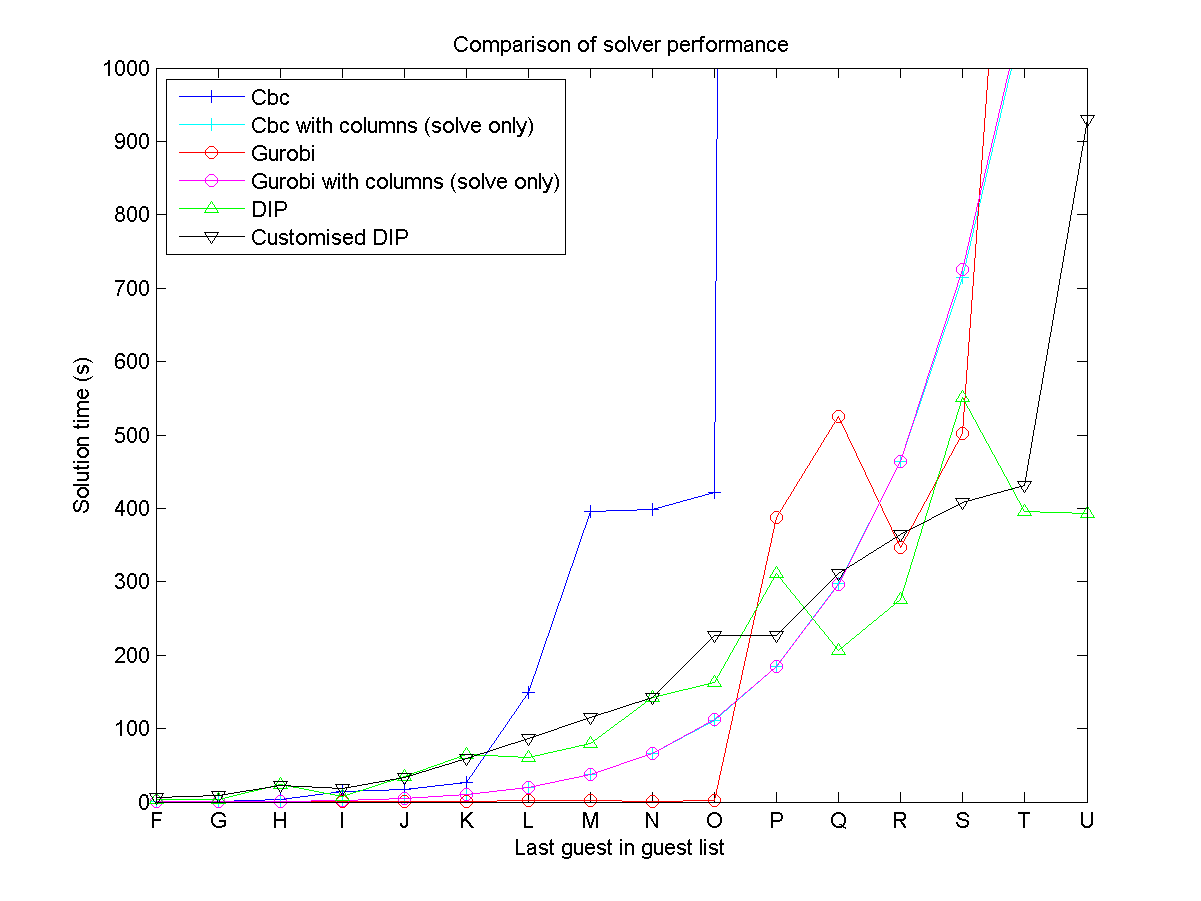
\includegraphics[bb=0 0 1201 901,scale=0.335]{compare.png}
\caption{Comparing solver performance on the Wedding Planner problem} \label{fig:compare}
\end{figure}
Thus, Dippy and \ac{DIP} not only provide a vastly simplified way to experiment with advanced \ac{MILP} techniques, they provide a better solver for problems in which column generation is the preferred approach.

Dippy presents the best of both worlds. It provides a mathematical modelling framework that makes it easy to quickly formulate \ac{MILP} problems. It also makes it easy to quickly customise the \ac{MILP} solution framework to experiment with the effectiveness of advanced \ac{MILP} techniques for the problem being solved. We have used Dippy successfully to enable final year undergraduate students to experiment with advanced branching, cut generation, column generation and root/node heuristics. Dippy also provides a simple interface to \ac{DIP}, a state of the art, ``out of the box'' column generation solver. Dippy breaks down the barrier to the experimentation with and use of advanced \ac{MILP} approaches for both practitioners and researchers. This enables them to concentrate on furthering Operations Research knowledge and solve hard problems instead of spending time programming \ac{MILP} formulations in a low-level language.